\chapter{Dynamique des robots manipulateurs}
\label{sec:dynamic}

Chapitre en construction!

%%%%%%%%%%%%%%%%%%%%%%%%%%%%%%%%%%%%%%%%%%%%%%%%%%%%%%%%%%%
\section{Introduction}
%%%%%%%%%%%%%%%%%%%%%%%%%%%%%%%%%%%%%%%%%%%%%%%%%%%%%%%%%%%

\video{Dynamique des robots manipulateurs}{https://youtu.be/6z3grrVNBj4}

%%%%%%%%%%%%%%%%%%%%%%%%%%%%%%%%%%%%%%%%%%%%%%%%%%%%%%%%%%%
\section{Structure des équations des modèles dynamiques}
%%%%%%%%%%%%%%%%%%%%%%%%%%%%%%%%%%%%%%%%%%%%%%%%%%%%%%%%%%%
La forme la plus générique (pour un système continu) des équations différentielles représentant l'évolution d'un système dynamique dans le temps est les équations d'états:
%
\begin{align}
\dot{\col{x}} = f( \col{x}, \col{u})
\end{align}
%
où $\col{x}$ est un vecteur d'état, i.e. la mémoire ou les niveaux d'énergie du système, et $\col{u}$ est un vecteur des entrées du système. C'est la représentation qui est utilisée par les simulateurs numériques pour calculer des trajectoires, pour générer des diagrammes de phases, et par plusieurs méthodes numérique pour générer des lois de commandes ou des trajectoires. 

Lorsque le système dynamique à représenter est un système purement mécanique où les entrée sont des forces, comme c'est souvent le cas en robotique, il est possible d'utiliser une représentation plus spécifique avec une structure d'ordre 2 qui décrit la relation reliant les dérivées secondes des coordonnées (les accélérations) aux autres forces impliquées:
%
\begin{align}
\underbrace{
H(\col{q}) \col{\ddot{q}} + C(\col{q},\col{\dot{q}}) \col{\dot{q}} 
}_{ m \Vec{a}}
=  
\underbrace{
\col{f} 
}_{\Vec{f}}
\label{eq:mecdyn}
\end{align}
%
où $\col{q}$ est un vecteur de coordonnées généralisée (des positions linéaires ou angulaires qui caractérise la configuration du système mécanique), $H$ est une matrice d'inertie, $C$ est la matrice de coriolis et $\col{f}$ un vecteur des forces impliquée dans le système.

Il est souvent utile de décomposer $\col{f}$ ainsi pour représenter spécifiquement les types de forces impliquées dans le système:
%
\begin{align}
\underbrace{
H(\col{q}) \col{\ddot{q}} + C(\col{q},\col{\dot{q}}) \col{\dot{q}} 
}_{\text{effets inertiels}}
+ 
\underbrace{
d(\col{\dot{q}},\col{q}) 
}_{\text{forces dissipatrices}}
+ 
\underbrace{
\col{g}(\col{q}) 
}_{\text{forces conservatrices}}
= 
\underbrace{
B(\col{q}) \col{u} 
}_{\text{effet des actionneurs}}
+
\underbrace{
J^T(\col{q}) \col{f}_e
}_{\text{force externes}}
\label{eq:manipulator}
\end{align}
%
Cette équation est parfois appelé l'équation des manipulateurs et cette représentation est très utile pour analyser le comportement de système robotique et synthétiser des lois de commandes.



%%%%%%%%%%%%%%%%%%%%%%%%%%%%%%%%%%%%%%%%%%%%%%%%%%%%%%%%%%%
\section{Équation des manipulateurs}
\label{sec:manipeq}
%%%%%%%%%%%%%%%%%%%%%%%%%%%%%%%%%%%%%%%%%%%%%%%%%%%%%%%%%%%

L'équation des manipulateur caractérise la dynamique d'un système robotique décrite dans l'espace des coordonnées des joints:
%
\begin{align}
H(\col{q}) \col{\ddot{q}} + C(\col{q},\col{\dot{q}}) \col{\dot{q}} + d(\col{q}, \col{\dot{q}}) + \col{g}(\col{q}) = B(\col{q}) \col{u}  + J^T(\col{q}) \col{f}_e
\label{eq:manipulator}
\end{align}
%
où $\col{q}$ est le vecteur des forces généralisée, $H$ est la matrice d'inertie, $C$ est la matrice des forces de Coriolis/centrifuge, $\col{d}$ est un vecteur de force dissipatrices, $\col{g}$ un vecteur de forces conservatrices (typiquement la gravité), $B$ est une matrice qui transforme le vecteur des forces des actionneurs $\col{\tau}$ en forces généralisée, et $J^T$ la transposée de la matrice jacobienne associée au point d'application d'une force externe $\col{f}_e$.

\begin{table}[htbp]
	\centering
	\caption{Nomenclature pour la dynamique dans l'espace des joints}	% Table caption must be placed on top of the table %
		\begin{tabular}{ c c l r }
        \hline \hline
				\multicolumn{4}{c}{Entiers} \\
				\hline \hline
			$n$             &  :  & nombre de DDL et de coordonnées généralisées                                         & \\
			$m$             &  :  & nombre d'actionneur                                       & \\
			$c$             &  :  & nombre de contraintes de contact                             & \\
			$o$             &  :  & nombre de coordonnée de l'espace de la tâche                        & \\ 
			\hline \hline
			\multicolumn{4}{c}{Vecteurs} \\
			\hline \hline
			$\col{u}$    &  :  & Forces/couples des actionneurs                                   & $m$  \\
            $\col{\tau}$    &  :  & Forces des actionneurs transformées en coordonnées généralisées                              & $n$  \\
			$\col{q}$       &  :  & Coordonnées généralisée / espace des joints    & $n$  \\
			$\col{c}$       &  :  & Force dissipatrices                             & $n$  \\
			$\col{g}$       &  :  & Force conservatrices                              & $n$  \\
			$\col{c}$       &  :  & Sommes des forces internes                 & $n$  \\
			$\col{\phi}$    &  :  & Contraintes                                          & $c$  \\
			$\col{f}_c$     &  :  & Forces de contact                                     & $c$  \\
			$\col{f}_{E_robot/env}$     &  :  & Forces cartésienne externe appliquée sur l'effecteur du robot                  & $o$  \\
			$\col{r}$       &  :  & Position de l'effecteur / coordonnées de l'espace de la tâche                             & $o$  \\
			\hline \hline
			\multicolumn{4}{c}{Matrices} \\
			\hline \hline
			$H$             &  :  & Matrice d'inertie                                            & $n$ x $n$ \\
			$C$             &  :  & Matrice de coriolis                       & $n$ x $n$ \\
			$B$             &  :  & Matrice des actionneurs                                & $n$ x $m$ \\
			$J$             &  :  & Matrice jacobienne de l'effecteur & $o$ x $n$ \\
			$J_c$           &  :  & Matrice jacobienne des contacts                        & $c$ x $n$  \\
		\hline \hline
        \end{tabular}		
	\label{tab:nom}
\end{table}

Parfois pour allégé la manipulation des équations, une version abrégée où $\col{c}$ est parfois utilisé pour regrouper toute les forces internes (qui sont des fonctions des états du systèmes):
%%%%%%%%%%%%%%%%%%%%%%%
\begin{align}
\col{c} = C(\col{q},\col{\dot{q}}) \col{\dot{q}} + d(\col{q}, \col{\dot{q}}) + \col{g}(\col{q})
\end{align}
%%%%%%%%%%%%%%%%%%%%%%%
ce qui simplifie, pour un cas sans forces externes, l'équation des manipulateurs à:
%%%%%%%%%%%%%%%%%%%%%%%
\begin{align}
H \col{\ddot{q}} + \col{c} = \col{\tau} 
\label{eq:manipulator_short}
\end{align}
%%%%%%%%%%%%%%%%%%%%%%%





\subsection{Systèmes de coordonnées additionnels}
\label{sec:coord}

Parfois il peut être utile de travailler avec des systèmes de coordonnées supplémentaire à l'espace des joints. La Figure \ref{fig:coord} montre quelques espaces supplémentaires qui peuvent être utilisés. 
%
\begin{figure}[H]
	\centering
		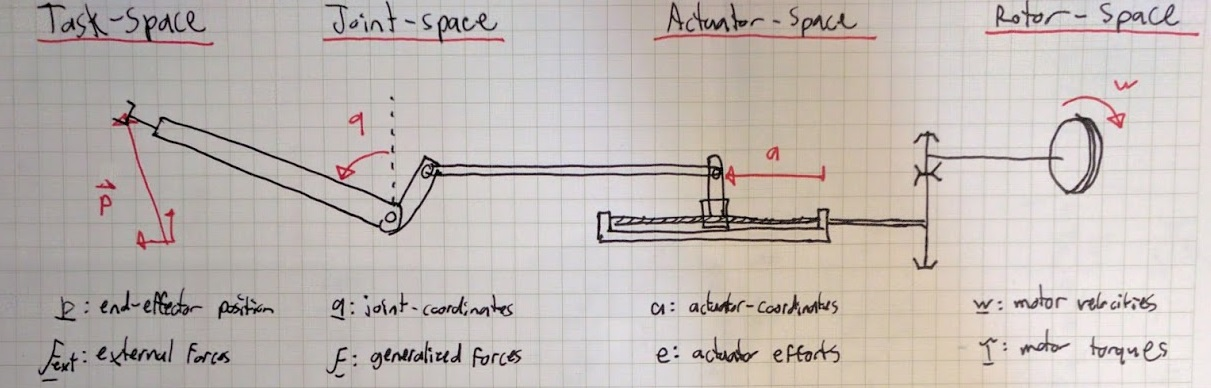
\includegraphics[width=0.99\textwidth]{coord.jpg}
	\caption{Coordinate systems}%
	\label{fig:coord}
\end{figure}
%
Si les relations cinématiques entre les coordonnées de ces espaces sont donné par:
%
\begin{align}
\col{\dot{r}}   &= J_e( \col{q} ) \col{\dot{q} }  \quad \text{ de l'espace des joints vers l'espace de la tâche   } \\
\col{\dot{a}}   &= J_a( \col{q} ) \col{\dot{q} }  \quad \text{ de l'espace des joints vers l'espace des actionneurs } \\
\col{w }        &= R              \col{\dot{a} }  \quad\quad \text{ de l'espace des actionneurs vers l'espace des moteurs } 
\label{eq:coord_transform2}
\end{align}
%
%
On pourrait utiliser ces relations pour inclure directement des forces dans l'espace des actionneurs $\col{f}_a$, et définir $\col{\tau}$ comme les couples moteurs plutôt celui rapporté au joint ainsi:
%
\begin{align}
H \col{\ddot{q}} + C \col{\dot{q}} + \col{d} + \col{g} =  \underbrace{ J_a^T(\col{q}) R^T }_{B(\col{q})}  \col{\tau} + J_e^T(\col{q}) \col{f}_e + J_a^T(\col{q}) \col{f}_a
\label{eq:manipulator_gen}
\end{align}

\subsection{Matrice des actionneurs}

La matrice $B(q)$ est une matrice de transformation qui relie le vecteur $\tau$,  représentants les entrées de notre système, et les forces généralisées associées dans le systèmes de coordonnées $\col{q}$ utilisé pour décrire les équations. La Figure \ref{fig:actuatormatrix} illustre qualitativement divers architecture d'actionneurs qui mène à différentes structures pour $B$:
%%%%%%%%%%%%%%%%%%%%%%%%%%%%%%%%%%%%%%%%%%%%%%%%%%%%%%%%%%%%%%%%%%%%%%%%%%%%
\begin{figure}[H]
	\centering
		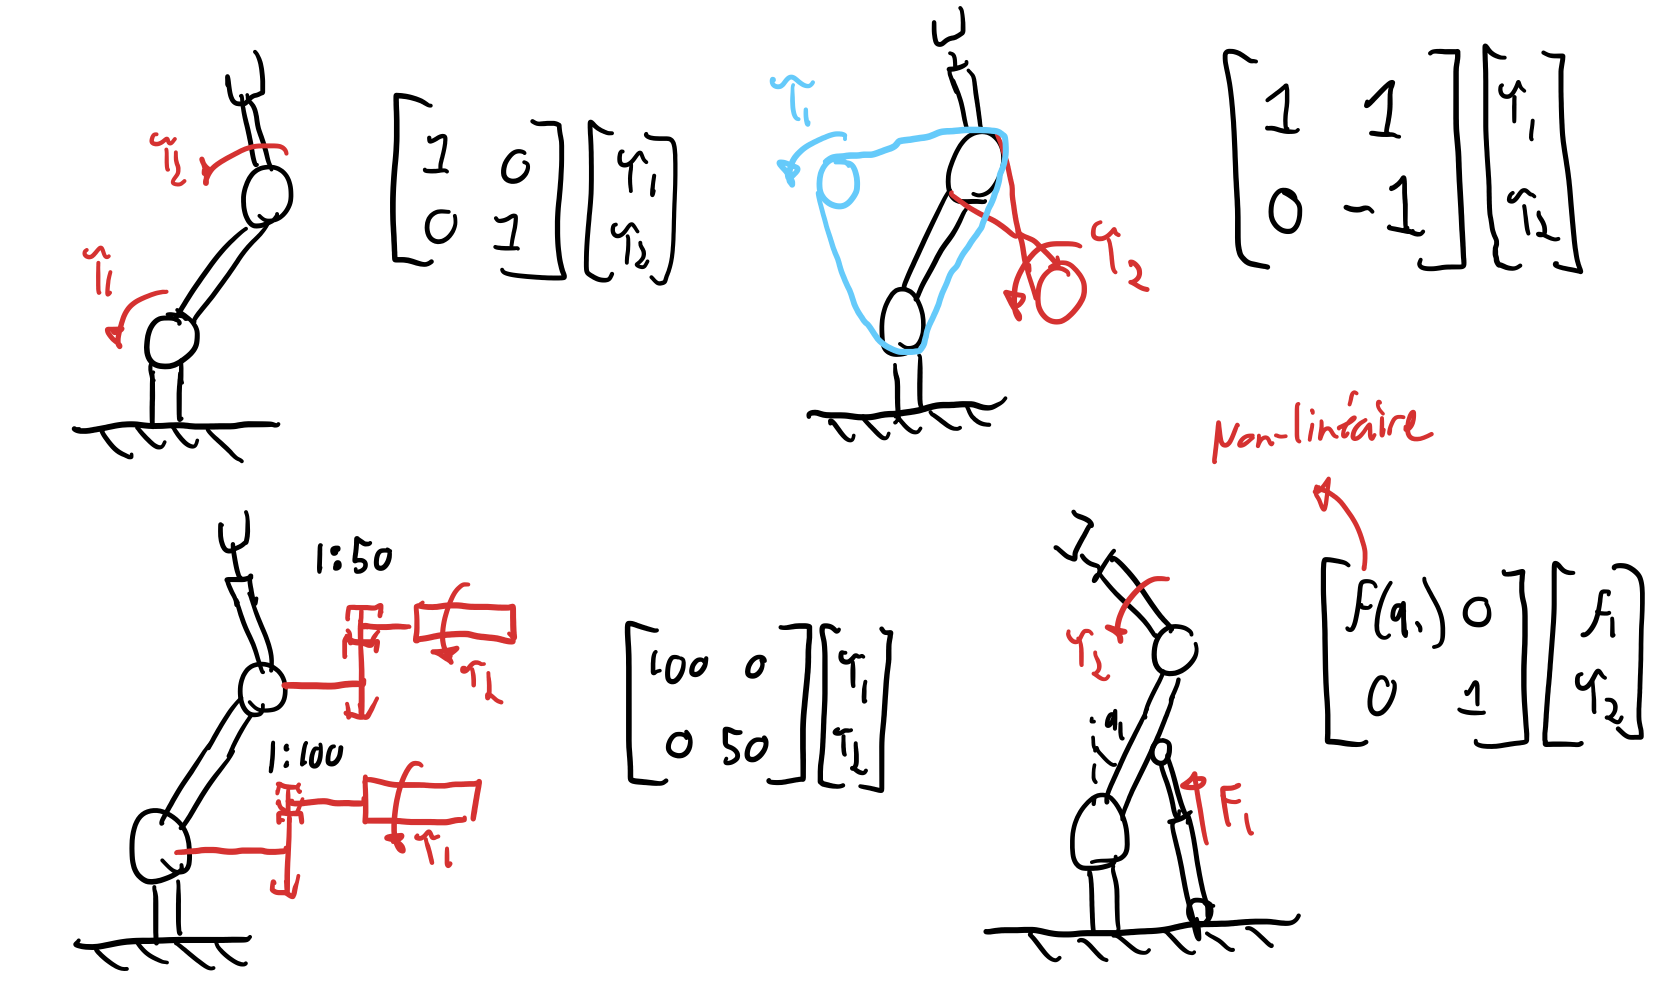
\includegraphics[width=0.70\textwidth]{fig/actuatormatrix.png}
	\caption{Matrice $B$ des actionneurs}%
	\label{fig:actuatormatrix}
\end{figure}
%%%%%%%%%%%%%%%%%%%%%%%%%%%%%%%%%%%%%%%%%%%%%%%%%%%%%%%%%%%%%%%%%%%%%%%%%%%%

Le cas le plus simple est lorsque les entrées $\tau$ sont des forces colocalisées avec les coordonnées généralisées $\col{q}$, par exemple si $\tau$ représente des couples net aux joint d'un système alors la matrice $B$ est la matrice identité.

La notion de puissance est utile pour définir cette matrice: le produit scalaire entre le vecteur vitesse des coordonnées généralisée $\col{\dot{q}}$ et les forces généralisées associées aux actionneurs $B\col{\tau}$ correspond à la puissance entrante fournit par les actionneurs:
%
\begin{align}
P_{actionneur} = \col{\dot{q}}^T B\col{\tau}
\end{align}


\subsection{Forces externes}

Voir section \ref{sec:manipstatic}. 

\subsection{Forces conservatrices}

Voir section \ref{sec:manipstaticconservative}. 


\subsection{Forces dissipatrices}

%
\begin{align}
\dot{Q}_{out} = \dot{\col{q}}^T \col{d}
\end{align}
%

\subsection{Effets inertiels}
%
L'énergie cinétique du système est directement reliée à la matrice d'inertie $H$ et la vitesse des joints $\dot{\col{q}}$:
%
\begin{align}
\frac{1}{2} \col{\dot{q}}^T H(\col{q}) \col{\dot{q}} 
\label{eq:kinetic}
\end{align}
%
La matrice $C$ n'est pas une propriété indépendante du système, elle est en fait reliée à la variation temporelle de la matrice $H$:
%
\begin{align}
\dot{H} = C + C^T
\label{eq:cener}
\end{align}

%
% TODO la version indicielle


\subsection{Conservation de l'énergie}

\begin{align}
\frac{dE}{dt}     &= P_{in} - P_{out} \\
\dot{T} + \dot{V}  &= \sum \tau_i \dot{q}_i  - \sum f_i \dot{r}_i - \dot{Q} \\
\frac{d}{dt}\left( \frac{1}{2} \col{\dot{q}}^T H \col{\dot{q}} \right) + \frac{\partial V}{\partial \col{q}^T} \dot{\col{q}} &= \col{\tau}^T \col{\dot{q}}  - \col{f}_e^T J \col{\dot{q}} - \col{d}^T \col{\dot{q}}
\end{align}

\begin{align}
\dot{\col{q}}^T \left[ H \col{\ddot{q}} + \frac{1}{2}\dot{H}\dot{\col{q}} + \frac{\partial V}{\partial \col{q}^T} + \col{d} - \col{\tau} - J^T \col{f}_e  \right] &= 0 \\
\dot{\col{q}}^T \left[ \frac{1}{2}\dot{H} - C \right] \dot{\col{q}} &= 0
\end{align}




\newpage
%%%%%%%%%%%%%%%%%%%%%%%%%%%%%%%%%%%%%%%%%%%%%%%%%%%%%%%%%%%
\section{Équations avec la méthode de Lagrange}
\label{sec:lagrange}
%%%%%%%%%%%%%%%%%%%%%%%%%%%%%%%%%%%%%%%%%%%%%%%%%%%%%%%%%%%

\video{Méthode de Lagrange pour déterminer les équations dynamiques}{https://youtu.be/AUcs0L85liM}



\newpage
%%%%%%%%%%%%%%%%%%%%%%%%%%%%%%%%%%%%%%%%%%%%%%%%%%%%%%%%%%%
\section{Équations dans l'espace de la tâche}
\label{sec:taskdynamics}
%%%%%%%%%%%%%%%%%%%%%%%%%%%%%%%%%%%%%%%%%%%%%%%%%%%%%%%%%%%

\begin{align}
H \col{\ddot{q}} + \col{c} = \col{\tau} 
\label{eq:manipulator_short2}
\end{align}

%%%%%%%%%%%%%%%%
\begin{align}
\col{r} &= f\left( \, \col{q} \, \right) \\
\col{\dot{r}} &= J\left( \, \col{q} \, \right) \, \col{\dot{q}} \\
\col{\ddot{r}} &= J\left( \, \col{q} \, \right) \, \col{\ddot{q}}  + \dot{J} \left( \, \col{q}  , \col{\dot{q}} \, \right) \, \col{\dot{q}} 
\end{align}
%%%%%%%%%%%%%%%


\newpage
%%%%%%%%%%%%%%%%%%%%%%%%%%%%%%%%%%%%%%%%%%%%%%%%%%%%%%%%%%%
\section{Manipulateur en contact avec l'environnement}
\label{sec:contact}
%%%%%%%%%%%%%%%%%%%%%%%%%%%%%%%%%%%%%%%%%%%%%%%%%%%%%%%%%%%

Cette section présente les outils pour obtenir les équations du mouvement lorsqu'un système robotique est en contact avec l'environnement, ce qui contraint sont mouvement. 

\subsubsection{Contraintes cinématique}
\label{sec:constraints}
%
SI un robot manipulateur est en contact avec un objet fixe, il pert certains DDL. Dans le cas de contraintes bilatérales, la contrainte peut être décrite par une fonction:
\begin{align}
\col{\phi}( \col{ q } ) = 0
\label{eq:constraint}
\end{align}
%
Si on dérive cette fonction par rapport au temps, il est possible d'obtenir des conditions pour la vitesse et l'accélération du système:
\begin{align}
\frac{d \col{\phi}( \col{ q } ) }{dt}     &= J_c( \col{ q } ) \col{\dot{q}}  = 0 \\
\frac{d^2 \col{\phi}( \col{ q } ) }{dt^2} &= J_c( \col{ q } ) \col{\ddot{q}}  + \dot{J}_c( \col{ q } ) \col{\dot{q}} = 0 
\label{eq:constraint_diff}
\end{align}
%
où $J_c$ est le jacobien des contraintes:
%
\begin{align}
J_c( \col{ q } )                    &= \frac{d \col{\phi}( \col{ q } ) }{d\col{ q }}
\label{eq:constraint_jaco}
\end{align}

\subsubsection{Forces de contraintes}
\label{sec:constraint_forces}

Le jacobien des contraintes peut être utilisé pour transformer des forces de contact cartésiennes $\col{f}_c$ en force généralisée au joint dans l'équation des manipulateurs:
%
\begin{align}
H \col{\ddot{q}} + \col{c} = B \col{\tau} + J_c( \col{ q } )^T  \col{f}_c
\label{eq:manipulator_constraint}
\end{align}
%
Si on isole $\col{\ddot{q}}$ dans l'équation \eqref{eq:manipulator_constraint} pour ensuite substituer dans l'équation \eqref{eq:constraint_diff}, on retrouve une expression des forces de contraintes qui dépend des états actuel du système et des forces/couples aux actionneurs:
%
\begin{align}
\col{f}_c = \left( J_c H^{-1} J_c^T \right)^{-1} \left(  J_c H^{-1} [\col{c} - B \col{\tau} ] - \dot{J}_c( \col{ q } ) \col{\dot{q}}   \right)
\label{eq:const_forces}
\end{align}
%
Alternativement il est possible, pour trouver l'accélération $\col{\ddot{q}}$ et les forces de contact $\col{f}_c$ simultanément, de résoudre le système d'équation suivant:
%
\begin{align}
\left[ \begin{array}{c c } 	H & -J_c^T  \\ J_c 	& 0  	\end{array} \right] \left[ \begin{array}{c} \col{\ddot{q}}  \\ \col{f}_c \end{array} \right] = \left[ \begin{array}{c}  B \col{\tau} - \col{c}   \\ -\dot{J}_c \col{\dot{q}}  \end{array} \right]
\label{eq:manipulator_constraint_eom}
\end{align}


\subsubsection{Impulsion lors d'un impact}
\label{sec:impact}
%
Quand le robot rentre en contact avec un objet fixe très rigide (frapper le sol par exemple), des forces de contact impulsives vont agir sur le système. Si on intègre l'équation \eqref{eq:manipulator_constraint} sur une période infinitésimal de temps $dt$ donne:
%
\begin{align}
\int{ ( H \col{\ddot{q}} + \col{c} ) dt } &= \int{ ( B \col{\tau} + J_c( \col{ q } )^T  \col{f}_c ) dt } \\
H \col{\dot{q}}^+ - H \col{\dot{q}}^- &= J_c( \col{ q } )^T  \int{  \col{f}_c dt }
\label{eq:manipulator_impact}
\end{align}
%
où la contribution des forces non-impulsive est négligée. Si on projette ces équations sur les coordonnées contraintes en multipliant par $J_c H^{-1}$ on trouve:
%
\begin{align}
J_c \col{\dot{q}}^+ - J_c \col{\dot{q}}^- &= J_c H^{-1} J_c^T  \int{  \col{f}_c dt }
\label{eq:manipulator_impact2}
\end{align}
%
Si on fait l'hypothèse d'une collision complètement inélastique (sans rebond), la contrainte est respectée à l'instant $t^+$ qui suit immédiatement l'impact. Dons comme $J_c \col{\dot{q}}^+=0$, il est ensuite possible de résoudre pour obtenir l'impulsion due au contact dans ces conditions:
\begin{align}
\int{  \col{f}_c dt } &= - \left( J_c H^{-1} J_c^T \right)^{-1}  J_c \col{\dot{q}}^-
\label{eq:manipulator_impact_force}
\end{align}
%
et pour la vitesse des joints qui va suivre immédiatement l'impact:
%
\begin{align}
\col{\dot{q}}^+ &= - \Big[ I - H^{-1} J_c^T \left( J_c H^{-1} J_c^T \right)^{-1} J_c \Big] \col{\dot{q}}^-
\label{eq:manipulator_impact_velocity}
\end{align}
%
ou pour la variation de vitesse durant l'impulsion:
%
\begin{align}
\Delta \col{\dot{q}} &=  \Big[ H^{-1} J_c^T \left( J_c H^{-1} J_c^T \right)^{-1} J_c \Big] \col{\dot{q}}^-
\label{eq:manipulator_impact_velocity_delta}
\end{align}
%
On peut alternativement résoudre le système de $n+c$ équations suivant pour obtenir ces résultats simultanément:
%
\begin{align}
\left[ \begin{array}{c c } 	H & -J_c^T  \\ J_c 	& 0  	\end{array} \right] \left[ \begin{array}{c} \col{\dot{q}}^+  \\ \int{ \col{f}_c dt }\end{array} \right] = \left[ \begin{array}{c}  	H \col{\dot{q}}^-   \\ 0  \end{array} \right]
\label{eq:manipulator_impact_eom}
\end{align}






\newpage
\section{Représentation des systèmes hybrides}

Hybrid dynamical system can be represented in the general form:
%
\begin{align}
\text{Continuous evolution: } \left(  \dot{\col{x}} , \dot{k} \right) &=  \left( \, f_k( \col{x} , \col{u} , \col{d} ) \, , \, 0 \, \right) \\
\text{Discrete jumps: } \left(  \col{x}^+ , k^+ \right) &=  \left( h_{ij}( \col{x}^- , \col{u}^- ) , j \right) \quad\text{if}\quad \left(  \col{x} , k , \col{u} \right) \in D_{ij}  
\end{align}
%
where $\col{x}$ is a continuous state vector, and $k$ is a discrete mode and $D_{ij}$ is the domain mapping conditions leading to a transition $k:i \rightarrow j$. For robotic systems, the discrete mode can represent discrete configurations of the robot , like discrete modes in the control law or contact/non-contact conditions. The jump map then represents the impulsive response when contact is made. 

\subsection{Switched system}

A restricted class of hybrid system, called switched system, are hybrid systems for which the jump map for continuous state is the identify function:
%
\begin{align}
\text{Continuous evolution: } \left(  \dot{\col{x}} , \dot{k} \right) &=  \left( \, f_k( \col{x} , \col{u} , \col{d} ) \, , \, 0 \, \right) \\
\text{Discrete jumps: } \left(  \col{x}^+ , k^+ \right) &=  \left( \col{x}^- , j \right) \quad\text{if}\quad \left(  \col{x} , k , \col{u} \right) \in D_{ij} 
\end{align}
%

\subsubsection{Switched system where the discrete mode is a control input}

In the situation where the discrete operating mode $k$ is a control input, then there is no need to keep track of discrete mode evolution and only the piece-wise continuous differential equations are sufficient to model the system evolution:
%
\begin{align}
\dot{\col{x}} = f_k( \col{x} , \col{u} , \col{d} ) 
\end{align}
%
A robot with a continuous dynamics but with a control law using discrete modes of operation would be of this category. 








% BACKUP ENG

\iftoggle{EN}{%
\section{Equations of motion in joint-space}
%\section{Équations du mouvement dans l'espace des joints}
\label{sec:eom}

The general form of the equations of motion of robotic systems (interconnected rigid body driven by motors) is:
%
\begin{align}
H(\col{q}) \col{\ddot{q}} + C(\col{q},\col{\dot{q}}) \col{\dot{q}} + D \col{\dot{q}} + \col{g}(\col{q}) = B(\col{q}) \col{\tau} 
\label{eq:manipulator}
\end{align}
%
where $\col{q}$ is the generalized coordinates vector, $H$ is the inertia matrix, $C$ is the Coriolis/centrifugal force matrix, $D$ is a damping matrix, $\col{g}$ is the gravitational forces vector and $B$ is a matrix mapping motor torques $\col{\tau}$ into generalized forces.
%
Kinetic energy is given by:
%
\begin{align}
\frac{1}{2} \col{\dot{q}}^T H(\col{q}) \col{\dot{q}} 
\label{eq:kinetic}
\end{align}
%
Conservation of energy also give the following relation:
%
\begin{align}
\dot{H} = C + C^T
\label{eq:cener}
\end{align}
%
On occasion, dependence notation is dropped and $\col{c}$ is used to represent all state dependent forces, leading to the short form:
%
\begin{align}
H \col{\ddot{q}} + \col{c} = B \col{\tau} 
\label{eq:manipulator_short}
\end{align}

\begin{table}[htbp]
	\centering
	\caption{Nomenclature pour la dynamique dans l'espace des joints}	% Table caption must be placed on top of the table %
		\begin{tabular}{ c c l r }
        \hline \hline
				\multicolumn{4}{c}{Scalars} \\
				\hline \hline
			$n$             &  :  & number of DoF                                              & \\
			$m$             &  :  & number of actuators                                        & \\
			$c$             &  :  & number of contact constraints                              & \\
			$o$             &  :  & number of end-effector coordinates                         & \\ 
			$i$             &  :  & index for DoF                                              & \\ 
			\hline \hline
			\multicolumn{4}{c}{Vectors} \\
			\hline \hline
			$\col{\tau}$    &  :  & Actuator forces/torques                                    & $m$  \\
			$\col{q}$       &  :  & Joint coordinates position vector                          & $n$  \\
			$\col{w}$       &  :  & Actuator coordinates velocity vector                          & $m$  \\ 
			$\col{g}$       &  :  & Gravitational forces vector                                & $n$  \\
			$\col{c}$       &  :  & Sum of state-dependent generalized forces                  & $n$  \\
			$\col{\phi}$    &  :  & Constraint vector                                          & $c$  \\
			$\col{f}_c$     &  :  & Contact forces vector                                      & $c$  \\
			$\col{f}_e$     &  :  & End-effector external forces vector                        & $o$  \\
			$\col{r}$       &  :  & End-effector position vector                               & $o$  \\
			\hline \hline
			\multicolumn{4}{c}{Matrices} \\
			\hline \hline
			$H$             &  :  & Inertia matrix                                             & $n$ x $n$ \\
			$D$             &  :  & Damping matrix                                             & $n$ x $n$ \\
			$C$             &  :  & Coriolis/Centrifugal forces matrix                         & $n$ x $n$ \\
			$B$             &  :  & Generalized forces matrix                                  & $n$ x $m$ \\
			$J_a$           &  :  & Actuator coordinates / joint coordinates Jacobian matrix   & $m$ x $n$ \\
			$J_e$           &  :  & Task-space coordinates / joint coordinates Jacobian matrix & $o$ x $n$ \\
			$J_c$           &  :  & Contact constraints Jacobian matrix                        & $c$ x $n$  \\
		\hline \hline
        \end{tabular}		
	\label{tab:nom}
\end{table}




Fig. \ref{fig:coord} shows all the used coordinates systems. 
%
\begin{figure}[H]
	\centering
		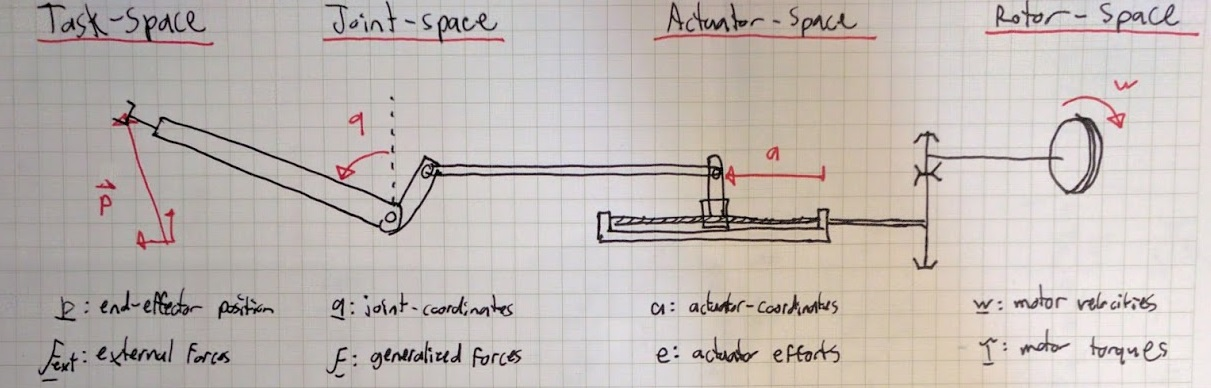
\includegraphics[width=0.99\textwidth]{coord.jpg}
	\caption{Coordinate systems}%
	\label{fig:coord}
\end{figure}
%
Where coordinates transforms are defined by:
%
\begin{align}
\col{\dot{r}}   &= J_e( \col{q} ) \col{\dot{q} }  \quad \text{ from joint-space to end-effector   } \\
\col{\dot{a}}   &= J_a( \col{q} ) \col{\dot{q} }  \quad \text{ from joint-space to actuator-space } \\
\col{w }        &= R              \col{\dot{a} }  \quad\quad \text{ from actuator-space to rotor-space } 
\label{eq:coord_transform2}
\end{align}
%
%
The following equation represents the most general case:
%
\begin{align}
H \col{\ddot{q}} + C \col{\dot{q}} + D \col{\dot{q}} + \col{g} =  \underbrace{ J_a^T(\col{q}) R^T }_{B(\col{q})}  \col{\tau} + J_e^T(\col{q}) \col{f}_e + J_c^T(\col{q}) \col{f}_c
\label{eq:manipulator_gen}
\end{align}


\newpage
\section{Contact}
\label{sec:contact}

This section presents equations for representing contact situations.

\subsubsection{Kinematic constraints}
\label{sec:constraints}
%
If a robotic manipulator enter contact with a fixed object, then some DoF are constrained. In the case of a bilateral constraint, the constraint can be expressed as:
\begin{align}
\col{\phi}( \col{ q } ) = 0
\label{eq:constraint}
\end{align}
%
The time-derivative of the constraint must also be equal to zero, which gives some constraints in terms of velocity and acceleration:
\begin{align}
\frac{d \col{\phi}( \col{ q } ) }{dt}     &= J_c( \col{ q } ) \col{\dot{q}}  = 0 \\
\frac{d^2 \col{\phi}( \col{ q } ) }{dt^2} &= J_c( \col{ q } ) \col{\ddot{q}}  + \dot{J}_c( \col{ q } ) \col{\dot{q}} = 0 
\label{eq:constraint_diff}
\end{align}
%
when $J_c$ is the constraint Jacobian:
%
\begin{align}
J_c( \col{ q } )                    &= \frac{d \col{\phi}( \col{ q } ) }{d\col{ q }}
\label{eq:constraint_jaco}
\end{align}

\subsubsection{Constraint forces}
\label{sec:constraint_forces}

The constraint Jacobian can be used to map constraint forces $\col{f}_c$ to generalized forces in the EoM:
%
\begin{align}
H \col{\ddot{q}} + \col{c} = B \col{\tau} + J_c( \col{ q } )^T  \col{f}_c
\label{eq:manipulator_constraint}
\end{align}
%
Solving for $\col{\ddot{q}}$ in eq. \eqref{eq:manipulator_constraint} and substituting in eq. \eqref{eq:constraint_diff}, it is possible to get and expression for the constraint forces $\col{f}_c$ as a function of states and applied torques:
%
\begin{align}
\col{f}_c = \left( J_c H^{-1} J_c^T \right)^{-1} \left(  J_c H^{-1} [\col{c} - B \col{\tau} ] - \dot{J}_c( \col{ q } ) \col{\dot{q}}   \right)
\label{eq:const_forces}
\end{align}
%
Alternatively, it possible to solve for acceleration $\col{\ddot{q}}$ and constraints forces $\col{f}_c$ simultaneously by solving the following system of equations:
%
\begin{align}
\left[ \begin{array}{c c } 	H & -J_c^T  \\ J_c 	& 0  	\end{array} \right] \left[ \begin{array}{c} \col{\ddot{q}}  \\ \col{f}_c \end{array} \right] = \left[ \begin{array}{c}  B \col{\tau} - \col{c}   \\ -\dot{J}_c \col{\dot{q}}  \end{array} \right]
\label{eq:manipulator_constraint_eom}
\end{align}


\subsubsection{Impact impulsive behavior}
\label{sec:impact}
%
When the robot first enters contact with a fixed object, impulsive contact forces will act on the system. Integrating eq. \eqref{eq:manipulator_constraint} over the short impact interval gives:
%
\begin{align}
\int{ ( H \col{\ddot{q}} + \col{c} ) dt } &= \int{ ( B \col{\tau} + J_c( \col{ q } )^T  \col{f}_c ) dt } \\
H \col{\dot{q}}^+ - H \col{\dot{q}}^- &= J_c( \col{ q } )^T  \int{  \col{f}_c dt }
\label{eq:manipulator_impact}
\end{align}
%
where any non-impulsive forces are neglected during the short impact interval. Projecting onto constrained coordinates (multiplying by $J_c H^{-1}$) gives:
%
\begin{align}
J_c \col{\dot{q}}^+ - J_c \col{\dot{q}}^- &= J_c H^{-1} J_c^T  \int{  \col{f}_c dt }
\label{eq:manipulator_impact2}
\end{align}
%
Then assuming a sticky inelastic impact (no bouncing), then the constraint is respected after the impact ($J_c \col{\dot{q}}^+=0$) and it is possible to solve for the impact force:
%
\begin{align}
\int{  \col{f}_c dt } &= - \left( J_c H^{-1} J_c^T \right)^{-1}  J_c \col{\dot{q}}^-
\label{eq:manipulator_impact_force}
\end{align}
%
and also for the velocity after the impact:
%
\begin{align}
\col{\dot{q}}^+ &= - \Big[ I - H^{-1} J_c^T \left( J_c H^{-1} J_c^T \right)^{-1} J_c \Big] \col{\dot{q}}^-
\label{eq:manipulator_impact_velocity}
\end{align}
%
Or change in velocity:
%
\begin{align}
\Delta \col{\dot{q}} &=  \Big[ H^{-1} J_c^T \left( J_c H^{-1} J_c^T \right)^{-1} J_c \Big] \col{\dot{q}}^-
\label{eq:manipulator_impact_velocity_delta}
\end{align}
%

Alternatively, it possible to solve for velocity $\col{\dot{q}}^+$ and impulsive forces $\int{ \col{f}_c dt }$ simultaneously by solving the following system of $n+c$ equations:
%
\begin{align}
\left[ \begin{array}{c c } 	H & -J_c^T  \\ J_c 	& 0  	\end{array} \right] \left[ \begin{array}{c} \col{\dot{q}}^+  \\ \int{ \col{f}_c dt }\end{array} \right] = \left[ \begin{array}{c}  	H \col{\dot{q}}^-   \\ 0  \end{array} \right]
\label{eq:manipulator_impact_eom}
\end{align}


\section{Hybrid system dynamics}

Hybrid dynamical system can be represented in the general form:
%
\begin{align}
\text{Continuous evolution: } \left(  \dot{\col{x}} , \dot{k} \right) &=  \left( \, f_k( \col{x} , \col{u} , \col{d} ) \, , \, 0 \, \right) \\
\text{Discrete jumps: } \left(  \col{x}^+ , k^+ \right) &=  \left( h_{ij}( \col{x}^- , \col{u}^- ) , j \right) \quad\text{if}\quad \left(  \col{x} , k , \col{u} \right) \in D_{ij}  
\end{align}
%
where $\col{x}$ is a continuous state vector, and $k$ is a discrete mode and $D_{ij}$ is the domain mapping conditions leading to a transition $k:i \rightarrow j$. For robotic systems, the discrete mode can represent discrete configurations of the robot , like discrete modes in the control law or contact/non-contact conditions. The jump map then represents the impulsive response when contact is made. 

\subsection{Switched system}

A restricted class of hybrid system, called switched system, are hybrid systems for which the jump map for continuous state is the identify function:
%
\begin{align}
\text{Continuous evolution: } \left(  \dot{\col{x}} , \dot{k} \right) &=  \left( \, f_k( \col{x} , \col{u} , \col{d} ) \, , \, 0 \, \right) \\
\text{Discrete jumps: } \left(  \col{x}^+ , k^+ \right) &=  \left( \col{x}^- , j \right) \quad\text{if}\quad \left(  \col{x} , k , \col{u} \right) \in D_{ij} 
\end{align}
%

\subsubsection{Switched system where the discrete mode is a control input}

In the situation where the discrete operating mode $k$ is a control input, then there is no need to keep track of discrete mode evolution and only the piece-wise continuous differential equations are sufficient to model the system evolution:
%
\begin{align}
\dot{\col{x}} = f_k( \col{x} , \col{u} , \col{d} ) 
\end{align}
%
A robot with a continuous dynamics but with a control law using discrete modes of operation would be of this category. 


}{}